\section{Test}
Durante il lavoro di tesi sono stati svolti alcuni test. 
Sono stati eseguiti su una macchina con sistema operativo Windows 10, un processore Intel Core i7 6700HQ a 2.60GHz (6M Cache, up to 3.50 GHz) e con 16Gb di RAM DDR4.

Si possono evidenziare 4 gruppi:
\begin{itemize}
    \item Test per il Reverse Engineering
    \item Test di integrità 
    \item Test di prestazione
    \item Test di rilassamento
\end{itemize}

\subsection{Test di Reverse Engineering}
Il progetto riguardante la ricerca di dipendenze funzionali rilassate non possedeva una documentazione esaustiva. Per tale motivo si è deciso di creare delle classi Test, che avessero il compito di mostrare il processo effettuato da ogni modulo.
Le classi di test create sono:
\begin{itemize}[noitemsep]
\let\labelitemi\labelitemii
    \item diff{\_}test.py : utilizzata per comprendere il funzionamento della classe che genera la matrice delle differenze.
    \item relaxer{\_}test.py: utilizzata per testare la classe QueryRelaxer.
    \item rfd{\_}extractor{\_}test.py utilizzata per testare il modulo che funge da Bridge per l'algoritmo di ricerca di RFD.
\end{itemize}

\subsection{Test di integrità}
Durante lo sviluppo sono state create delle classi per il testing. Seppur non paragonabili a dei test di unità sono state utili per controllare il funzionamento di ogni singolo modulo.
\begin{itemize}[noitemsep]
\let\labelitemi\labelitemii
    \item io{\_}test.py: utilizzata per testare la classe RFDInputOutput().
    \item csv{\_}parser{\_}test.py: utilizzata per controllare il corretto funzionamento della classe CSVParser. 
    \item csv{\_}test.py: utilizzata per controllare la corretta estrazione dell'header.
    \item dataframe{\_}row{\_}slicer{\_}test.py: utilizzata per controllare il corretto funzionamento della classe Slicer.
    \item similar{\_}strings{\_}test.py: utilizzata per testare la funzionalità di ricerca di stringhe simili.
\end{itemize}
\subsection{Test di prestazione}
Per misurare le prestazioni non è stato creato un modulo ad hoc, bensì sono stati eseguiti due gruppi di test manuali:
Il primo gruppo di test è servito a testare la bontà dell'ordinamento delle RFD. 
Un buon ordinamento di RFD deve porre prima le RFD che ampliano il Result Set di poco,
in modo tale da evitare di produrre un Result Set che contengano dati poco inerenti all'interrogazione iniziale.
Per effettuare questo controllo sono stati dichiarate tre variabili:
\begin{itemize}
    \item original{\_}query{\_}result{\_}set{\_}size: una variabile che contiene la cardinalità del Result Set restituito inizialmente.
    \item relaxed{\_}query{\_}result{\_}set{\_}size: una variabile che contiene la cardinalità del Result Set restituito dalla query rilassata.
    \item dataset{\_}size: una variabile che contiene la cardinalità del DataSet.
\end{itemize}
Si è deciso di applicare un' ottimizzazione sulla ricerca dell'RFD migliore. 
Ogni volta che viene effettuata una Query Rilassata, prima restituire il Result Set, vengono testate le prime N RFD.
Grazie a questi variabili è possibile controllare quanto aumenta la cardinalità del Result Set per ogni RFD. Viene quindi restituita l'RFD che produce il Result Set meno ampio possibile che sia però maggiore del Result Set restituito dalla query iniziale. In questo modo si cercano di ottenere i risultati che siano maggiormente correlati con l'interrogazione iniziale.

Il secondo gruppo di test è stato eseguito verificare quanto tempo chiedesse l'algoritmo.
Si è deciso di non tener conto dei tempi di ricerca/caricamento delle RFD, in quanto non dipendono direttamente dal lavoro sviluppato.

\begin{figure}[H]
    \centering
    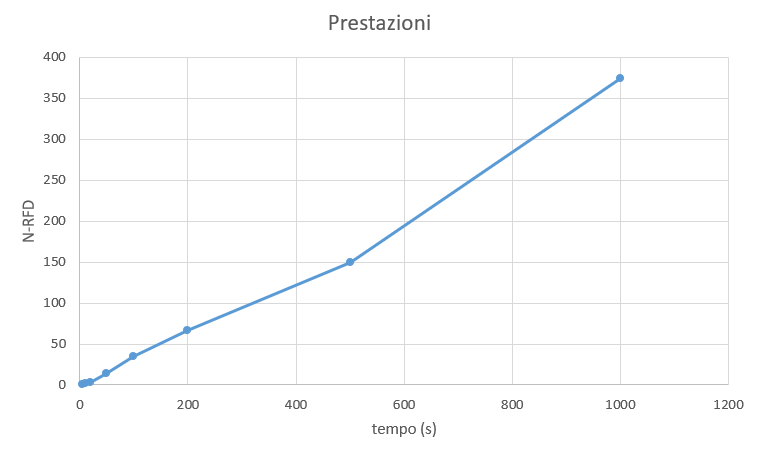
\includegraphics[width=\textwidth,height=\textheight,keepaspectratio]{Prestazioni.PNG}
    \caption{Prestazioni}
    \label{fig:prestazioni}
\end{figure}

\begin{figure}[H]
    \centering
    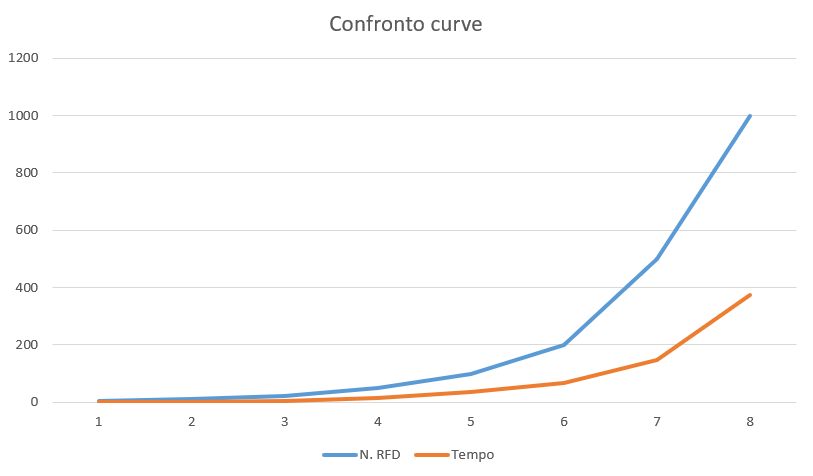
\includegraphics[width=\textwidth,height=\textheight,keepaspectratio]{confronto_curve.PNG}
    \caption{Confronto tra curve}
    \label{fig:confronto_curve}
\end{figure}

\subsection{Test di rilassamento}
Sono stati effettuati vari test su diversi Database per testare la qualità dei Result Set prodotti dal rilassamento delle query.

Un esempio significativo è quello eseguito sul DataSet in figura
\begin{figure}[H]
    \centering
    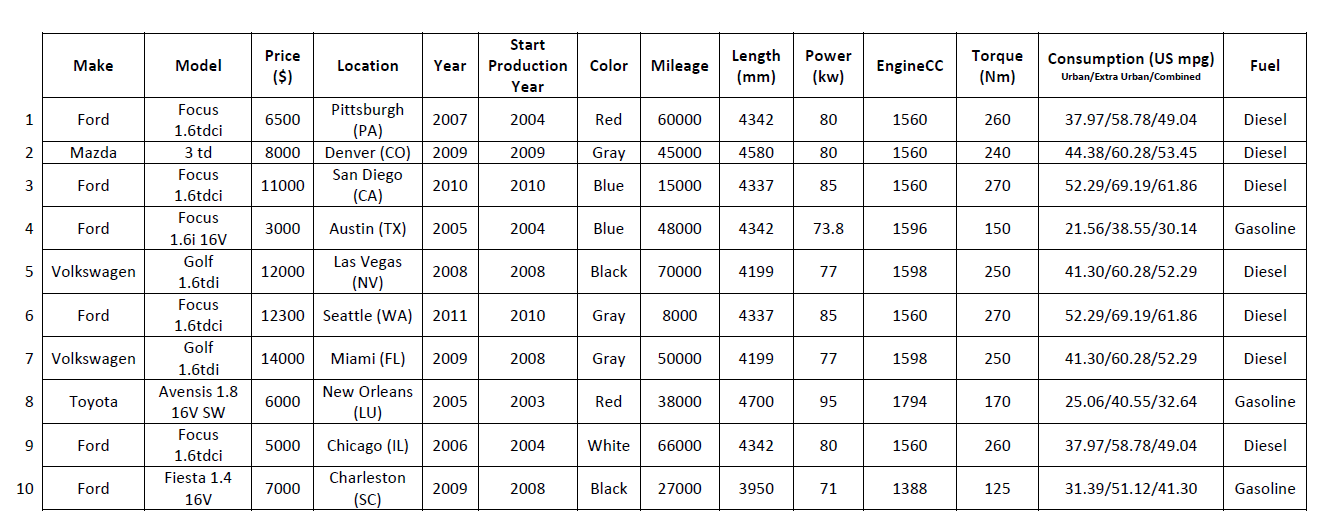
\includegraphics[width=\textwidth,height=\textheight,keepaspectratio]{DB.PNG}
    \caption{DataSet cars{\_}db.csv}
    \label{fig:dataset_cars_db}
\end{figure}

Inizialmente è stata eseguita la query:
\begin{center}
FROM cars{\_}db.csv WHERE Model LIKE \lq\%Focus\%\rq
AND Price $\geq$ 7500 AND Price $\leq$ 8500
\end{center}

Il Result Set prodotto da questa query è vuoto, in quanto nel DataSet non è presenta alcuna tupla che soddisfa tali vincoli.
Utilizzando il software di Query Relaxation sviluppato viene individuata l'RFD migliore.
\begin{center}
$(mileage \leq 3801.0) (model \leq 5.0) (price \leq 1700.0) \rightarrow (location \leq 8.0)$
\end{center}

Rilassando la query in base alle soglie della RFD il Result Set viene ampliato con successo, ottenendo il risultato maggiormente correlato con la query iniziale.
\begin{figure}[H]
    \centering
    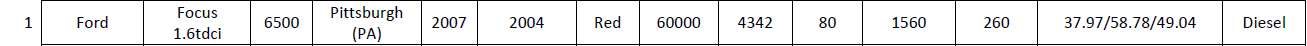
\includegraphics[width=\textwidth,height=\textheight,keepaspectratio]{DB_query_rs.PNG}
    \caption{Risultato query rilassata su cars{\_}db.csv}
    \label{fig:rs_query_rx_cars_db}
\end{figure}


Un ulteriore query interessante è quella eseguita su dataset{\_}string.csv
\begin{center}
FROM dataset{\_}string.csv WHERE name == \lq joh \rq
\end{center}

In questo caso il Result Set è vuoto in quanto non è presente alcuna tupla che rispetti tale vincolo.
Il software di Query Relaxation ha individuato come migliore la seguente query:
\begin{center}
    $(name \leq 1.0) \rightarrow (age \leq 1.0)$
\end{center}

Rilassando la query secondo le soglie della RFD viene restituito il seguente Result Set:
\begin{table}[H]
    \centering
    \begin{tabular}{|l |l |l |l |}
    \hline
    name & sex & city & age \\
    \hline
    john & male & newyork &  20 \\
    jack & male & newyork &  21 \\
    domenico & male & newyork &  21\\
    \hline
    \end{tabular}
    \caption{Result Set da query rilassata su dataset{\_}string.csv }
    \label{tab:ds_rx_query_ds_str}
\end{table}

È interessante notare che , in questo caso , un sistema di rilassamento banale avrebbe agito solo sul parametro \textit{name} , restituendo probabilmente solo le tuple riguardanti \quotes{john} e \quotes{jack}. \\
Mentre il sistema sviluppato è stato in grado di agire sul parametro \quotes{age} grazie alla conoscenza fornita dalla RFD.

Come ultimo esempio desidero includere un caso verificatosi nelle fasi iniziali di sperimentazione. Effettuando la query :
\begin{center}
FROM dataset{\_}string.csv WHERE name == \lq joh \rq
\end{center}
su dataset{\_}string.csv gli algoritmi di ordinamento restituivano come RFD migliore la seguente:
\begin{center}
    $(name \leq 3.0)  \rightarrow (sex \leq 0.0)$
\end{center}

Tale RFD aveva un problma, avendo attributo \quotes{sex} in RHS, nel momento in cui si rilassava la query, si interrogava il DataSet cercando tutte le tuple che contenessero valore \quotes{male} sull'attributo sex, ciò produceva un Result Set che era di cardinalità pari a metà del DataSet. Il DataSet è abbastanza piccolo, di conseguenza non vi erano molti problemi, ma ovviamente lo stesso problema si sarebbe potuto ripresentare un DataSet molto più ampi. Per ovviare a tale inconveniente sono stato introdotti alcuni controlli, in modo tale da scartare le RFD che producessero Result Set troppo ampi.


\section{Riflessioni}
Dopo aver completato la descrizione del progetto sviluppato è necessario fare qualche osservazione.
L'idea iniziale non è era quella di sviluppare un modulo professionale che permetta il rilassamento di query, ma lo scopo principale è stato quello di dimostrare che è possibile creare un sistema di rilassamento basato sulle RFD.
%DA AMPLIARE
Il sistema, seppur necessitante di diverse migliorie, è stato sviluppato in modo da essere facilmente manutenibile. 
Si può collegare facilmente il modulo ad un sistema di ricerca su Web, l'unica limitazione è data dalla poca scelta di comandi SQL, che sono però facilmente modificabili.
Il progetto ha richiesto circa due mesi di sviluppo per essere completato. Si è svolto sotto la supervisione del prof. Vincenzo Deufemia e della dott.ssa Loredana Caruccio. Il lavoro si è svolto con il collega Maurizio Casciano.

\section{Lavori futuri}
Seguono ora alcuni idee da implementare in futuro.
\paragraph{Preferenze utente}
Qualsiasi ordinamento di RFD che non tiene conto del grado di importanza degli attributi per l'utente, difficilmente produrrà un sistema che sia in grado di dare il risultato cercato.
Il problema consiste nell'impossibilità di verificare tutti i possibili legami che esistono all'interno di un Database, ed anche analizzandole tutte \footnote{In un universo in cui ciò sia fattibile.}, non è detto che l'RFD scelta restituirà il risultato cercato dall'utente. Perché ciò?
La questione sta nell'andare a intendere su che punto l'utente è disposto a cedere. Se inizialmente effettua una query contente tre attributi, l'utente magari su alcuni di essi è disposto ad essere flessibile, mentre su altri non vuole compromessi \footnote{Si pensi a quando si cerca un prodotto su di uno Store, quasi nessuno vuole compromessi sul parametro \quotes{prezzo}.}.
Si suggerisce quindi di implementare un sistema che permetta all'utente di specificare il grado di flessibilità di ogni parametro.
\paragraph{Sistema di query Simil-SQL}
Le attuali opzioni di query sono abbastanza scarne, è consigliabile implementare ulteriori opzioni, prendendo d'esempio quelle del SQL. In particolare servirebbero le opzioni: groupby,orderby,in,join.
Tranne la \quotes{join} che richiede una revisione della struttura del progetto, il resto è facilmente implementabile.
\paragraph{Parallelizzazione}
Tutto il progetto è stato sviluppato senza parallelizzazione. Sia l'ordinamento che la scelta della query rilassata è facilmente parallelizzabile. Ciò può portare ad un aumento delle prestazioni, di conseguenza diventa più semplice effettuare maggiori test sulle RFD, permettendo cosi di ottenere Result Set che siano di maggior interesse per l'utente.